\documentclass[10pt]{article}   	% use "amsart" instead of "article" for AMSLaTeX format
\usepackage{geometry}                		% See geometry.pdf to learn the layout options. There are lots.
\usepackage[english]{babel}
\geometry{a4paper}                   		% ... or a4paper or a5paper or ... 
%\geometry{landscape}                		% Activate for for rotated page geometry
%\usepackage[parfill]{parskip}    		% Activate to begin paragraphs with an empty line rather than an indent
\usepackage{graphicx}				% Use pdf, png, jpg, or epsß with pdflatex; use eps in DVI mode
\usepackage{fontspec}
\usepackage{multicol}
\setmainfont{Arial}
					
\linespread{1.1}			% TeX will automatically convert eps --> pdf in pdflatex		
\usepackage{amssymb}
\usepackage{eurosym}
\usepackage{colortbl}
\title{MorphicDraw}
\author{Stephan J.C. Eggermont, Sensus}
\begin{document}
\setlength{\parindent}{0pt}
\maketitle
\begin{quote}
\em
MorphicDraw is a drawing application demonstrating some of the power of Morphic.
Morphic is a powerful graphics environment, used in Self, Squeak, Cuis and Pharo.
In an iterative and incremental process, build up an application that supports
drawing connected figures.
\end{quote} 
%%%%%%%%%%%%%%%%%%%%%%%%%%%%%%%%%%%%%%%%%%%
\section{A Morphic Application with a Window}
\begin{figure}[htb]
\begin{center}
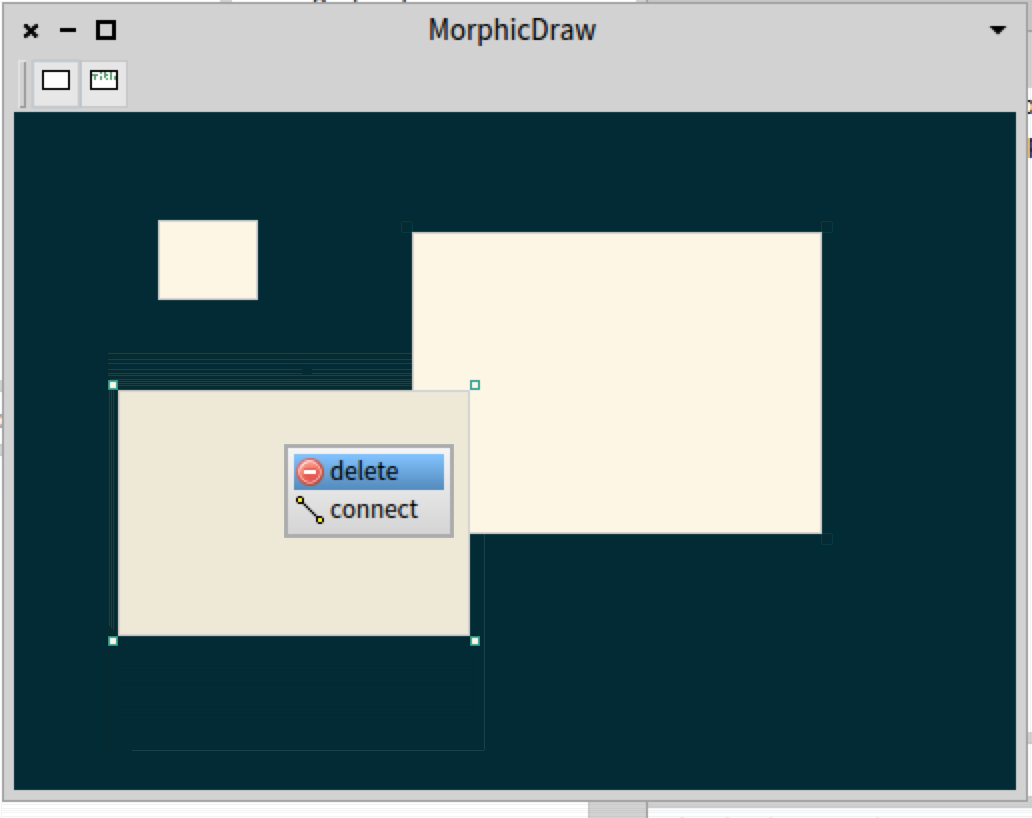
\includegraphics[width=200pt]{SimpleMorphicDrawWindow.png}
\caption{A first iteration of the main window of MorphicDraw}
\label{1stIteration}
\end{center}
\end{figure}
The first iteration (Figure \ref{1stIteration})  shows an application window 
with a toolbar and a drawing area. In the drawing area there are 
three graphical shapes, one of which is selected. A context menu
for the selected shape shows options to delete it and to connect it.

There are several frameworks build on top of basic Morphic that
help creating larger applications.
\begin{itemize}
\item Polymorph
\item Glamour
\item Spec
\end{itemize}
All three have their own documentation and examples. They can all 
be used with MorphicDraw.
\subsection{Using Polymorph}
Add a class that represents the application. It has instance variables for 
the different parts. 

\begin{verbatim}
Object subclass: #MorphicDraw
    instanceVariableNames: 'window tools dock'
    classVariableNames: ''
    category: 'MorphicDraw-Model'
\end{verbatim}

Creating a window in Polymorph (and Morphic)  is simple. Open a workspace and DoIt
\begin{verbatim}
StandardWindow new openInWorld 
\end{verbatim} 
This creates a window and opens it on the screen. 
It already has default behaviour for closing and resizing, and a default title. 
All graphical elements in Morphic are subclasses of Morph, and the 
World is a container for all of them. Opening a Morph in the world
positions it and makes it visible. An alternative to opening it directly is
to add it to the (mouse) cursor. In Morphic this is called the hand.
DoIt:
\begin{verbatim}
StandardWindow new openInHand 
\end{verbatim} 
The window is then positioned by clicking.

The MorphicDraw application uses the first, but needs to change 
the window title. It will grow its size to fit the contents.

\begin{verbatim}
MorphicDraw>>createWindow
    window := StandardWindow new
        setLabel: 'MorphicDraw';
        yourself.
\end{verbatim}

StandardWindow is part of Polymorph. Polymorph extends Morphic
with theme-ability. PolyMorph widgets often strictly adhere to the theme,
ignoring the Morphic-level setters for colors and borders defined in
their superclassses.  Polymorph makes the 
Window responsible for adding predefined user interface widgets
to the application Window. For that it uses the TEasilyThemed 
trait. It adds a lot (163 in my current image) of convenience methods.

In Morphic, a toolbar in a window has buttons on it. This iteration of
MorphicDraw uses two buttons to be able to create two different 
graphical shapes.

\begin{verbatim}
MorphicDraw>>createNewCardButton
    ^ window
        newButtonFor: self
        getState: nil
        action: #newCard
        arguments: nil
        getEnabled: nil
        labelForm: MDIcons default cardIcon
        help: 'New Card' translated
\end{verbatim}
The help text is shown when hovering the mouse over the button.
The button is always enabled, and sends the \#newCard message 
without any arguments to self when it is pressed. It has no 
state-dependent behaviour or shape. The icon for the button
is provided by MDIcons default cardIcon (see the Icons section,  p. \pageref{Icons}).

The button for the other shape is similar:
\begin{verbatim}
MorphicDraw>>createNewRectangleButton
    ^ window
        newButtonFor: self
        getState: nil
        action: #newRectangle
        arguments: nil
        getEnabled: nil
        labelForm: MDIcons default rectangleIcon
        help: 'New Rectangle' translated
\end{verbatim}

The newCard and newRectangle are implemented by creating a
new morph of the right kind and opening it in the hand. Both MDShape is a
subclass of BorderedMorph and MDCard a subclass of MDShape.

\begin{verbatim}
MorphicDraw>>newCard
    ^MDCard new openInHand

MorphicDraw>>newRectangle
    ^MDShape new openInHand
\end{verbatim}

A toolbar in Morphic consists of two parts, a ToolDockingBar and
a Toolbar. The Toolbar is added to the dock. A DockingBarMorph 
sticks to one edge of the Morph that it is added to.

\begin{verbatim}
MorphicDraw>>createToolBar
    tools := window newToolbar: 
        (Array with: self createNewRectangleButton with: self createNewCardButton).
    dock := window newToolDockingBar.
    dock addMorph: tools
\end{verbatim}
This allows the creation and opening of the window
\begin{verbatim}
MorphicDraw>>open
     self createWindow.
     self createToolBar.
     window
         addMorph: dock
            fullFrame: ((0@0 corner: 1@0) asLayoutFrame bottomOffset: dock minExtent y);
        addMorph: MDPanel new 			
            fullFrame: ((0@0 corner: 1@1) asLayoutFrame topOffset: dock minExtent y).
    ^window openInWorld.
\end{verbatim}
Some morphs automatically lay out their submorphs when they are added,
others need to add an explicit layout strategy. The toolbar adds its toolbar buttons
from left to right without a gap between them.  
The toolbar dock by default takes up the top edge of the morph it is added to. 
For a window that is the area with the drag bar, title and window icons. 
A LayoutFrame that should fit the whole contents area of the window is
created using a rectangle from 0@0 to 1@1.
\begin{verbatim}
(0@0 corner: 1@1) asLayoutFrame.   
\end{verbatim}
The left half would be (0@0 corner: 0.5@1).
Space can be left at a side by using the bottom/top/left/rightOffset.
The dock knows its minimum height
\begin{verbatim}
dock minExtent y
\end{verbatim}
so uses a layout frame based on the top line, extending it at its bottom
by the dock height. The MDPanel is a PasteUpMorph subclass containing
all the drawing shapes.

At the class side add a method to open the application

\begin{verbatim}
MorphicDraw>>open
    ^self new open
\end{verbatim}
%%%%%%%%%%%%%%%%%%%%%%%%%%%%%%%%%%%%%%%%%%%
\subsection{Using Glamour}
Glamour is designed to quickly create different kinds of browsers.
It models a browser as consisting of panes that influence each other 
by their selection. 

Create a new class
\begin{verbatim}
Object subclass: #GlamourMorphicDraw
    instanceVariableNames: 'browser'
    classVariableNames: ''
    category: 'MorphicDraw-Model' 
\end{verbatim}
At the class side add a method to open the application
\begin{verbatim}
GlamourMorphicDraw class>>open
    ^self new open
\begin{verbatim}
A glamour browser is always opened on an object. 
Open on self, not on nil.
\begin{verbatim}
GlamourMorphicDraw >>open
    self browser openOn: self
\end{verbatim}
The browser itself is constructed in several steps:
\begin{itemize}
\item set the title;
\item define the (nested) rows and columns of panes.
This one is simple with only one element in one column.
\item for each pane, define what pane influences it. 
A transmission has a from and to, with the transmission from
the outside (\#openOn:) being ignored.
\item in the andShow: block define what is to be put in the
presentation (a). In this case, show the MDPanel morph.
\item and finally define the actions that can be performed
from this pane.
\end{itemize}
\begin{verbatim}
browser
    browser := GLMTabulator new.
    browser title: 'Glamour MorphicDraw'.
    browser column:#morph.
    browser transmit to: #morph; andShow: [ :a |
        a morph 
            title: 'Untitled';
            morph: [MDPanel new];
            act: [:text | MDShape new openInHand ] icon: MDIcons default rectangleIcon entitled: 'New rectangle';
            act: [:text | MDCard new openInHand ] icon: MDIcons default cardIcon entitled: 'New card'].
    ^browser
\end{verbatim}
The resulting glamour application (Figure \ref{glamour}) can be opened with a DoIt
\begin{verbatim}
GlamourMorphicDraw open
\end{verbatim}

\begin{figure}[htb]
\begin{center}
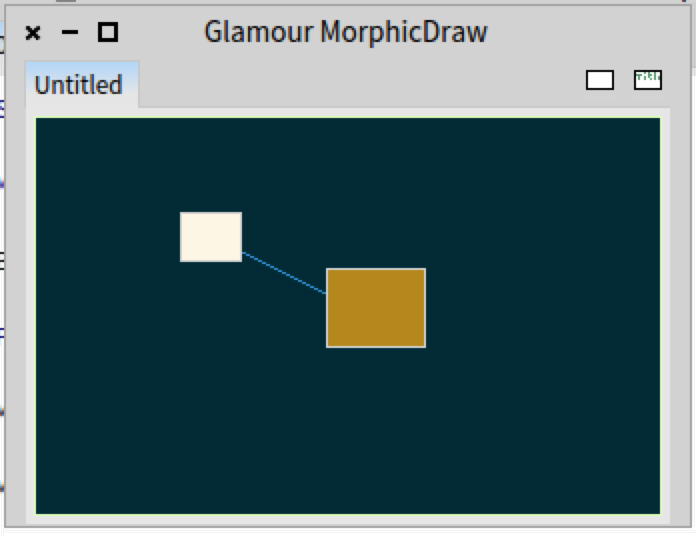
\includegraphics[width=200pt]{GlamourMorphicDraw.png}
\caption{MorphicDraw in Glamour}
\label{glamour}
\end{center}
\end{figure}
%%%%%%%%%%%%%%%%%%%%%%%%%%%%%%%%%%%%%%%%%%%
\section{Using Spec}
In Spec the application is a subclass of ComposableModel and holds onto the menu toolbar
and the panel morph.
\begin{verbatim}
ComposableModel subclass: #SpecMorphicDraw
    instanceVariableNames: 'menu panel'
    classVariableNames: ''
    category: 'MorphicDraw-Model'
\end{verbatim}
Spec based applications are opened by sending an instance \#openWithSpec.
\begin{verbatim}
SpecMorphicDraw class>>open
	^self new openWithSpec
\end{verbatim}
The layout definition in Spec is on the class side
\begin{verbatim}
SpecMorphicDraw class>>defaultSpec
    <spec: #default>
	
    ^ SpecLayout composed
        newColumn: [ :c | 
            c 
                add: #menu height: self toolbarHeight;
                add: #panel ];
        yourself
\end{verbatim}
On the instance side, getters for the widgets are needed. MDPanel has a default extent,
and its spec adapter needs to know it should fill all available space.
\begin{verbatim}
SpecMorphicDraw>>menu
    ^menu
	
SpecMorphicDraw>>panel
    |morph|
    morph := MDPanel new.
    ^ morph asSpecAdapter
        hSpaceFill;
        vSpaceFill;
        yourself
\end{verbatim}
The widgets need to be initialized. First the menu is build, then the panel is added
\begin{verbatim}
SpecMorphicDraw>>initializeWidgets
    menu := MenuModel new
        addGroup: [ :group |
            group addItem: [ :item |
                item
                    name: nil;
                    description: 'New rectangle';
                    icon: MDIcons default rectangleIcon;
                    action: [ MDShape new openInHand ] ].
            group addItem: [ :item |
                item 
                    name: nil;
                    description: 'New card';
                    icon: MDIcons default cardIcon;
                    action: [ MDCard new openInHand  ] ]].
		
    menu applyTo: self.
    self focusOrder add: self panel
\end{verbatim} 
The resulting spec application (Figure \ref{spec}) can be opened with a DoIt
\begin{verbatim}
SpecMorphicDraw open
\end{verbatim}

\begin{figure}[htb]
\begin{center}
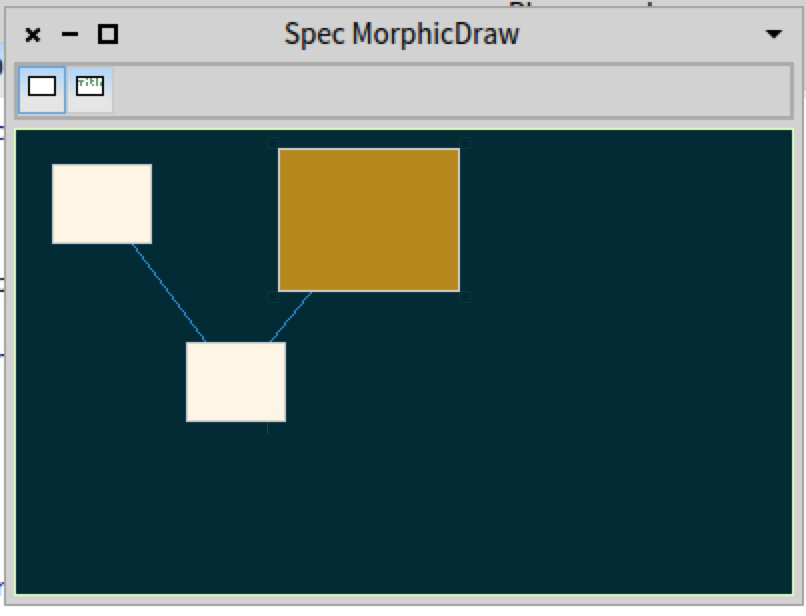
\includegraphics[width=200pt]{SpecMorphicDraw.png}
\caption{MorphicDraw in Spec}
\label{spec}
\end{center}
\end{figure}
%%%%%%%%%%%%%%%%%%%%%%%%%%%%%%%%%%%%%%%%%%%
\section{Shapes and PasteUpMorph}
The basic graphics entity in Morphic is a Morph. In a workspace, DoIt
\begin{verbatim}
Morph new openInWorld
\end{verbatim}
This opens a small blue rectangle on the screen. This can be dragged around on 
the screen. That is functionality that can be reused. World is a subclass of 
PasteUpMorph. The default PasteUpMorph is another small rectangle, this
time light green. 
\begin{verbatim}
PasteUpMorph new openInWorld
\end{verbatim}
After dragging a Morph onto a PasteUpMorph, it behaves as
a canvas containing the Morph. Let's use a subclass of PasteUpMorph
as the application canvas panel. 
\begin{verbatim}
PasteUpMorph subclass: #MDPanel
    instanceVariableNames: ''
    classVariableNames: ''
    category: 'MorphicDraw-Model'
\end{verbatim}
The default color for a PasteUpMorph is less suitable for MorphicDraw.
override it:
\begin{verbatim}
MDPanel>>defaultColor
    "answer the default color/fill style for the receiver"
    ^ MDColors base03
\end{verbatim}
Its default size is also too small.
\begin{verbatim}
MDPanel>>defaultBounds
"answer the default bounds for the receiver"
    ^ 0 @ 0 corner: 300 @ 200
\end{verbatim}

The method that decides what kind of Morphs a PasteUpMorph wants 
to receive is \#wantsDroppedMorph: aMorph event: evt. In WorldMorph this
always returns true, in PasteUpMorph only Morphs that are visible and
dropEnabled. MorphicDraw only wants to have to deal with its own 
Morphs. 
\begin{verbatim}
MDPanel>>wantsDroppedMorph: aMorph event: evt
    (aMorph isMorphicDraw) ifFalse: [ ^false ].
    ^super wantsDroppedMorph: aMorph event: evt
\end{verbatim}
This works by adding a method to a special protocol in Morph.
This is called creating an extension method.
In Morph add the protocol '*MorphicDraw-Model'.
In that protocol add a method
\begin{verbatim}
Morph>>isMorphicDraw
    ^false
\end{verbatim}
This method belongs to the MorphicDraw package, not to 
that of Morph, Morphic-Core.
A standard Morph has no border, this is added by BorderedMorph.
Create a subclass of BorderedMorph to use as the basic shape.
\begin{verbatim}
BorderedMorph subclass: #MDShape
    instanceVariableNames: 'selected highlighted connectors handles'
    classVariableNames: ''
    category: 'MorphicDraw-Model'
\end{verbatim}
and override isMorphicDraw
\begin{verbatim}
MDShape>>isMorphicDraw
    ^true
\end{verbatim}
Now test that the MDPanel only accepts MDShapes. 
DoIt
\begin{verbatim}
MDPanel new openInWorld.
MDShape new openInWorld.
\end{verbatim}
Verify that the shape can be dragged on the panel, and other morphs can not.
To make sure that an MDShape can only be dropped on a MDPanel,
add a method to MDShape
\begin{verbatim}
MDShape>>wantsToBeDroppedInto: aMorph
    ^aMorph class = MDPanel
\end{verbatim}

%%%%%%%%%%%%%%%%%%%%%%%%%%%%%%%%%%%%%%%%%%%
\section{Icons\label{Icons}}
The current icons in Pharo are bitmap icons. Athens makes it possible
to replace them by SVG, vector based icons. Polymorph adds the 
ThemeIcons class to make it easy to manage an applications' icons.
In this class a number of utility functions are defined to load and save
icons in png format. 

Create the png icons in an external program
(these were created with Gimp), store them in a directory.
Create a subclass of ThemeIcons
\begin{verbatim}
ThemeIcons subclass: #MDIcons
    instanceVariableNames: ''
    classVariableNames: ''
    category: 'MorphicDraw-Model'
\end{verbatim}
Add two methods containing the names for small- and normal sized icons
\begin{verbatim}
MDIcons>>normalSizeNames
    "Answer the names of the normal icons"
    ^#('rectangle' 'connector' 'card')

MDIcons>>smallSizeNames
    "Answer the names of the small icons. None"
    ^#()
\end{verbatim}
Provide a default instance of this class. At the class side, add 
a class instance variable and a lazy accessor
\begin{verbatim}
MDIcons class
    instanceVariableNames: 'default'

MDIcons class>>default
    ^default ifNil: [ ^self new ]
\end{verbatim}
Now add the icons using a utility method. In a workspace, DoIt
with directory replaced by the fully qualified path name of the
directory containing the icon png files:
\begin{verbatim}
MDIcons default createIconMethodsFromDirectory: directory 
\end{verbatim}
This adds two methods for each png file, one with a base64 encoded
contents and one icon form accessor. Form provides asMorph,
so the icons can be tested by DoIt
\begin{verbatim}
MDIcons default connectorIcon asMorph openInWorld
\end{verbatim}
This opens an ImageMorph with the icon in the World (Fig. \ref{iconhalos}). 
By selecting it with shift-alt, its halos are shown. With the cross halo the icon can be deleted. 
\begin{figure}[htb]
\begin{center}
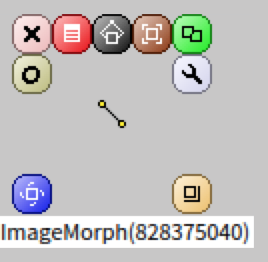
\includegraphics[width=150pt]{ImageIcon.png}
\caption{ImageMorph with icon and halos}
\label{iconhalos}
\end{center}
\end{figure}

By having the resource contents in a method, the normal version
control can be used and there is no need for specific resource
management. This works well when the resources are small and can be
manipulated in the image, like png icons.  

%%%%%%%%%%%%%%%%%%%%%%%%%%%%%%%%%%%%%%%%%%%
\section{Colors}
The responsibility for the colors used in MorphicDraw is given to the MDColors class.
This provides the actual colors. In a larger application, one would want to
separate these from their semantic use, so one would be able to use
 \#highlightColor or \#selectionColor, and make them dependent on the global
 setting of a dark or light theme.
\begin{verbatim}
Object subclass: #MDColors
    instanceVariableNames: ''
    classVariableNames: ''
    category: 'MorphicDraw-Model'
\end{verbatim}
At the moment there is no need to dynamically change these colors, so add
an indicator that the colors are all defined class-side.
\begin{verbatim}
MDColors>>seeClassSide
\end{verbatim}
At the class side, the colors for a Solarize color scheme are added
\begin{verbatim}
MDColors class>>base0
    ^Color fromHexString: '839496'

MDColors class>>base00
    ^Color fromHexString: '657b83'

MDColors class>>base01
    ^Color fromHexString: '586e75'
,,,
MDColors class>>red
    ^Color fromHexString: 'dc322f'

MDColors class>>violet
    ^Color fromHexString: '6c71c4'

MDColors class>>yellow
    ^Color fromHexString: 'b58900'
\end{verbatim}

%%%%%%%%%%%%%%%%%%%%%%%%%%%%%%%%%%%%%%%%%%%
\section{Selection and resizing}
Adding shapes to the panel and moving them around on it now works.
To manipulate shapes, Morphic by default uses halos. In this application
an approach more similar to drawing programs like Freehand or Illustrator
is preferred. When a shape is selected, show small manipulation squares
(handles) at the corners (Fig. \ref{selectedShape}) to be able to resize them.
\begin{figure}[htb]
\begin{center}
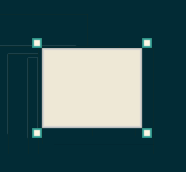
\includegraphics[width=150pt]{SelectedShape.png}
\caption{A selected shape}
\label{selectedShape}
\end{center}
\end{figure}
In the initialize of the MDShape the color and border color
are set.
\begin{verbatim}
MDShape>>initialize
    super initialize.
    self color: self defaultColor.
    self borderColor: self defaultBackgroundColor.
    selected := false.
    highlighted := false.
    connectors := OrderedCollection new.
    handles := OrderedCollection new.
    self on: #mouseUp send: #changeSelected to: self.
    self on: #mouseDown send: #startDrag:with: to: self.
    self on: #mouseMove send: #doDrag:with: to: self
\end{verbatim}
A new MDShape is not selected and not highlighted.
It has no connectors to other shapes and no handles.
The selection will be changed on \#mouseUp and 
the handles might have to be moved on \#mouseMove.
On \#mouseUp, the selection is changed and the shape
updates itself. 
\subsubsection{Constraining the drag to the panel}
On \#mouseDown, a drag might be started
and  that needs to be constrained to the panel.
The shape needs to know where the hand is dragging it. 
\begin{verbatim}
MDShape>>startDrag: evt with: dragHandle
    "Drag my target without removing it from its owner."
    super startDrag: evt with: dragHandle.
    ActiveHand addEventListener: self.
\end{verbatim}
and then
\begin{verbatim}
MDShape>>doDrag: aMouseMoveEvent with: aMDShape 
    ActiveHand addEventListener: self.
    self setConstrainedPosition: aMouseMoveEvent position - (self extent /2)hangOut: false.	
\end{verbatim}

\begin{verbatim}
MDShape>>changeSelected
    selected := selected not.
    self updateSelection. 
    ActiveHand removeEventListener: self.
\end{verbatim}
The color is changed to the color representing the 
selection state. Highlighting color dominates this color.
\begin{verbatim}
MDShape>>updateSelection
    selected ifTrue: [ 
        self color: self selectedColor.
        self showHandles]
    ifFalse: [ 
        self removeHandles.
        self color: self unselectedColor].
    highlighted ifTrue: [ 
        self color: self highlightColor  ]
\end{verbatim}
In showHandles, the morphs for the handles
are created the first time they are needed, then they are 
added to the shape and then (re)positioned on the respective
corners of the shape.
\begin{verbatim} 
MDShape>>showHandles
    handles ifEmpty: [ self addHandles ].
    handles do: [ :handle |
        self addMorph: handle ].
    self positionCorners
\end{verbatim}
Adding the handles consists of creating one with the
appropriate corner name.
\begin{verbatim}
MDShape>>addHandles
    #(topLeft bottomRight bottomLeft topRight) do: [ :aCorner | 
        handles add: (MDCornerHandle on: self at: aCorner) ].
\end{verbatim}
Positioning the corners is delegated to the handles
\begin{verbatim}
MDShape>>positionCorners
    handles do: [ :corner | corner rePosition ]
\end{verbatim}
\subsection{Corner handles}
A corner shape knows which corner of which subject it is for
\begin{verbatim}
BorderedMorph subclass: #MDCornerHandle
	instanceVariableNames: 'subject corner'
	classVariableNames: ''
	category: 'MorphicDraw-Model'
\end{verbatim}
The shape creates them
\begin{verbatim}
MDCornerHandle class>>on: aSubject at: aCorner
    "see instance side corners for possible values"
    ^self new
        subject: aSubject;
        corner: aCorner;
        yourself
\end{verbatim}
Because a morph shape responds to the corner name messages with
the position of the respective corner, \#reposition gets the location of
that corner from the subject
\begin{verbatim}
MDCornerHandle>>rePosition
    self positionMeAt: (subject perform: corner)
\end{verbatim}
To position the corner handle, all that is needed is the opposite
corner
\begin{verbatim}
MDCornerHandle>>oppositeCorners
    ^Dictionary newFromPairs:# (topLeft bottomRight: 
    leftCenter rightCenter: 
    bottomLeft topRight: 
    bottomCenter topCenter:
    bottomRight topLeft: 
    rightCenter leftCenter:
    topRight bottomLeft:
    topCenter bottomCenter:)
\end{verbatim} 
With that, the handle gets positioned exactly at the outside 
of the shape.
\begin{verbatim}
MDCornerHandle>>positionMeAt: aPosition
    self perform: (self oppositeCorners at: corner) with: aPosition
\end{verbatim}
To make sure that the corner handle can be used to scale its shape,
it needs to handle mouse events. Morphs only start receiving mouse
events if they declare their interest in them.
\begin{verbatim}
MDCornerHandle>>handlesMouseDown: evt
    ^true
\end{verbatim}
Once the mouse is moved, the subject needs to be resized to where
the mouse is and it needs to update the positions of the other corners.  
\begin{verbatim}
MDCornerHandle>>mouseMove: evt
    self reframedTo: evt position

MDCornerHandle>>reframedTo: aPoint	
    subject bounds: (subject bounds withSideOrCorner: corner setToPoint: aPoint).
    subject moved.
    subject positionCorners
\end{verbatim}
In \#moved the connectors can be updated.
\begin{verbatim}
MDShape>>moved
	connectors do: [ :connector | connector moved ]
\end{verbatim}
%%%%%%%%%%%%%%%%%%%%%%%%%%%%%%%%%%%%%%%%%%%
\section{Context menu}
The shape needs to react to mouse events. When the mouse button is pressed 
over the shape, it can be either part of a click or of the beginning of a drag.
The hand supports making that distinction. If the mouse is not moved too far
before the mouse button is released, it will send \#click: to the shape, otherwise
\#drag:with:.
\begin{verbatim}
MDShape>>mouseDown: evt
    evt ifNotNil: [  
        evt hand waitForClicksOrDrag: self event: evt]
\end{verbatim}
On a drag, the shape should be moved
\begin{verbatim}
MDShape>>doDrag: aMouseMoveEvent with: aMDShape 
    ActiveHand addEventListener: self.
    aMouseMoveEvent hand startDrag: aMouseMoveEvent with: aMDShape.
\end{verbatim}
The context menu is shown when the right button has been clicked.
No further propagation of the event is wanted.
\begin{verbatim}
MDShape>>click: evt
    "Default behavior: Show a context menu if right mouse button was clicked."
	
    evt yellowButtonPressed ifTrue: [
        self openContextMenuForHand: evt hand.
        evt wasHandled: true.]
\end{verbatim}
The context menu is a standard menu morph. It is filled with two
actions in menu items with icons: delete and connect. Both sent a message to the shape . 
By sending it \#popUpInWorld it is shown at the position of the hand. 
\begin{verbatim}
openContextMenuForHand: aHand
    | menu |
    menu := MenuMorph new defaultTarget: self.
    menu add: 'delete' selector: #delete;
        add: 'connect' selector: #connect.

    menu items first icon: Smalltalk ui theme icons deleteIcon .
    menu items second icon: MDIcons default connectorIcon .

    menu popUpInWorld
\end{verbatim}
%%%%%%%%%%%%%%%%%%%%%%%%%%%%%%%%%%%%%
\section{Connecting}
A PolygonMorph provides a good base for a connector.
Just add the shapes it connects to.
\begin{verbatim}
PolygonMorph subclass: #MDConnector
    instanceVariableNames: 'from to'
    classVariableNames: ''
    category: 'MorphicDraw-Model'
\end{verbatim}
A PolygonMorph supports both open 
figures and closed ones.Here it needs to be configured 
as a line-based polygon. It also supports both
smooth curves and ones with corners.
\begin{verbatim}
MDConnector>>initialize
    super initialize.
    closed := false.
\end{verbatim}
As the shapes keep track of their connectors, they need
to know when they are (dis)connected.
\begin{verbatim}
MDConnector>>from: anObject
    from ifNotNil: [ from connectors delete: self ].
    from := anObject.
    from connectors add: self.
    self moved.
\end{verbatim}
They connect from center to center of the shapes they connect to
and need to recalculate their shape when moved. Setting the 
vertices to an array with two points just creates a straight line.
\begin{verbatim}
MDConnector>>moved
    (from isNil | to isNil )ifFalse: [
    self vertices: (Array with: from center with: to center)]

MDConnector>>vertices: aCollection
	vertices := aCollection.
	self computeBounds
\end{verbatim}
This connector works fine when its two end-points are connected,
but has no support for creating a connection from one shape to 
another. For that to work the hand must be tracked from the
moment the connect action is started. A separate connector
type is used that deals with that.
\begin{verbatim}
MDShape>>connect
    |connector|
    connector := MDTempConnector from: self to: ActiveHand.
    connector openInWorld.
\end{verbatim}
This temporary connector should be able to highlight shapes it is 
over, to show where it can connect to.
\begin{verbatim}
MDConnector subclass: #MDTempConnector
    instanceVariableNames: 'over'
    classVariableNames: ''
    category: 'MorphicDraw-Model'
\end{verbatim}
It is connected to the active hand, and starts listening to
movements of the hand
\begin{verbatim}
MDTempConnector>>to: aHand
    to := aHand.
    ActiveHand addEventListener: self.
\end{verbatim}
It is only interested in mouse events. If it is moved it tries to find
a shape it is over and highlights it, and tries to make a connection 
on mouse up.
\begin{verbatim}
MDTempConnector>>handleListenEvent: anEvent
    anEvent isMouse ifFalse: [ ^self].
    anEvent isMouseUp ifTrue: [ self stopListening: anEvent]. 
    anEvent isMouseMove ifTrue: [ 
        self moved.
        self highlightShapeAt: anEvent ]
\end{verbatim}
On mouse up the event listener needs to stop listening, 
a highlighted shape is unhighlighted and the
temporary connector is removed. If the mouse up was over
a shape, it is replaced by a real connector.
\begin{verbatim}
MDTempConnector>>stopListening: anEvent
    ActiveHand removeEventListener: self.
    (self shapeAtPosition: anEvent) ifNotNil: [ :shape |
        from owner addMorphBack: (MDConnector from: from to: shape ) ].
    over ifNotNil: [ over unhighlight ].
    self delete
\end{verbatim}	
Morphic already support finding the morphs at a certain 
position. Select the shapes that can be connected to needs
an extra test that is returns false on Morph and true on
MDShape and subclasses.
\begin{verbatim}
MDTempConnector>>shapeAtPosition: anEvent
    "ask the panel instead of the world? 
    push up?"
    ^(World morphsAt: anEvent position) detect: [:aMorph |
        aMorph isMorphicDrawShape ] ifNone: [nil].
\end{verbatim}	
Highlight the right shape. The mouse can be moved 
both from shape to shape without moving over empty space.
\begin{verbatim}
MDTempConnector>>highlightShapeAt: anEvent
    |shape|
    shape := self shapeAtPosition: anEvent.
    over ifNil: [ 
        shape ifNotNil: [ 
            over := shape.
            over highlight ] ]
    ifNotNil: [ 
        shape = over ifFalse: [ 
            over unhighlight.
            over := shape.
            over ifNotNil: [  
            over highlight ] ] ]
\end{verbatim}	
%%%%%%%%%%%%%%%%%%%%%%%%%%%%%%%%%%%%%%%%%%%
\section{Z-order}
When adding shapes, the newest one gets to be in front. Morphs have a \#comeToFront
and \#goBehind method to change this order. Missing are up and down.
In the context menu add a submenu for this.
\begin{verbatim}
MDShape>>openContextMenuForHand: aHand
    | menu subMenu|
    menu := MenuMorph new defaultTarget: self.
    subMenu := MenuMorph new defaultTarget: self.
     subMenu add: 'to front' selector: #comeToFront;
        add: 'up' selector: #moveUp;
        add: 'down' selector: #moveDown;
        add: 'to back' selector: #goBehind.
	
    menu add: 'delete' selector: #delete;
        add: 'connect' selector: #connect;
        addLine;
        add: 'Z-order' subMenu: subMenu.
    menu items first icon: Smalltalk ui theme icons deleteIcon .
    menu items second icon: MDIcons default connectorIcon .

    menu popUpInWorld
\end{verbatim}

\#addMorph:asElementNumber: is guarded against adding beyond the number of 
submorphs, and removes the morph before reading it.
\begin{verbatim}
MDShape>>moveDown
    |ind|
    ind := self owner submorphIndexOf: self.
    self owner addMorph: self asElementNumber: ind + 1 

MDShape>>moveUp
    |ind|
    ind := self owner submorphIndexOf: self.
    ind > 1 ifTrue: [ self owner addMorph: self asElementNumber: ind - 1 ]
\end{verbatim}
%%%%%%%%%%%%%%%%%%%%%%%%%%%%%%%%%%%%%%%%%%%
\section{Selections}
Using shift-drag, a selection rectangle is created. It uses a SelectionMorph.
That needs some overrides to be usable with MDPanel. 

%%%%%%%%%%%%%%%%%%%%%%%%%%%%%%%%%%%%%%%%%%%
\section{Loading the code}
The code can be found on www.smalltalkhub.com, in the repository StephanEggermont/MorphicDraw
Open the Monticello Browser. Add a new repository of type smalltalkhub.com. 
The owner is StephanEggermont, the project is MorphicDraw. User and password are only needed
when you want to commit changes to the repository. Open the repository and load the latest version of
MorphicDraw.

\end{document}  